In leading order we have to consider photon-gluon-fusion (PGF), that is
\begin{equation}
\Pggx(q) + \Pg(k_1) \rightarrow \PQ(p_1)+\PaQ(p_2)
\end{equation}
with two contributing diagrams depicted in figure \ref{fig:FeynLO}.
\begin{figure}[ht!]
\centering
\begin{subfigure}[t]{.4\textwidth}
	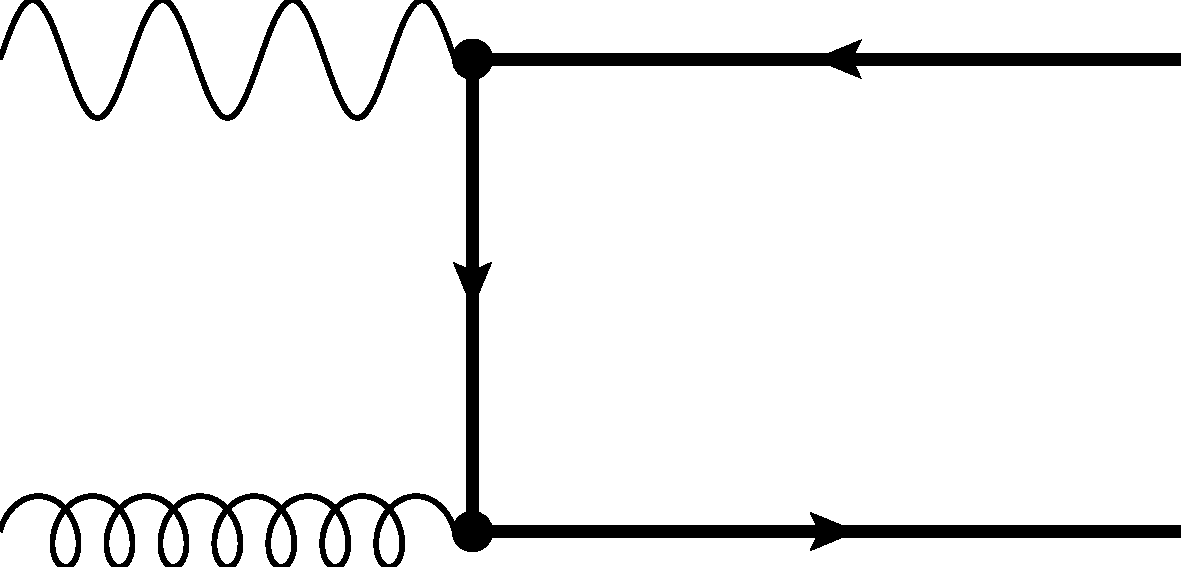
\includegraphics[width=\textwidth]{pyfeyn/lo-1}
	\caption{$i\varepsilon^{\mu}_{\Pgg}(q)\varepsilon^{\nu}_{\Pg}(k_1)\Md^{(0),1}_{\mu\nu}$}
\end{subfigure}\hspace{.15\textwidth}%
\begin{subfigure}[t]{.4\textwidth}
	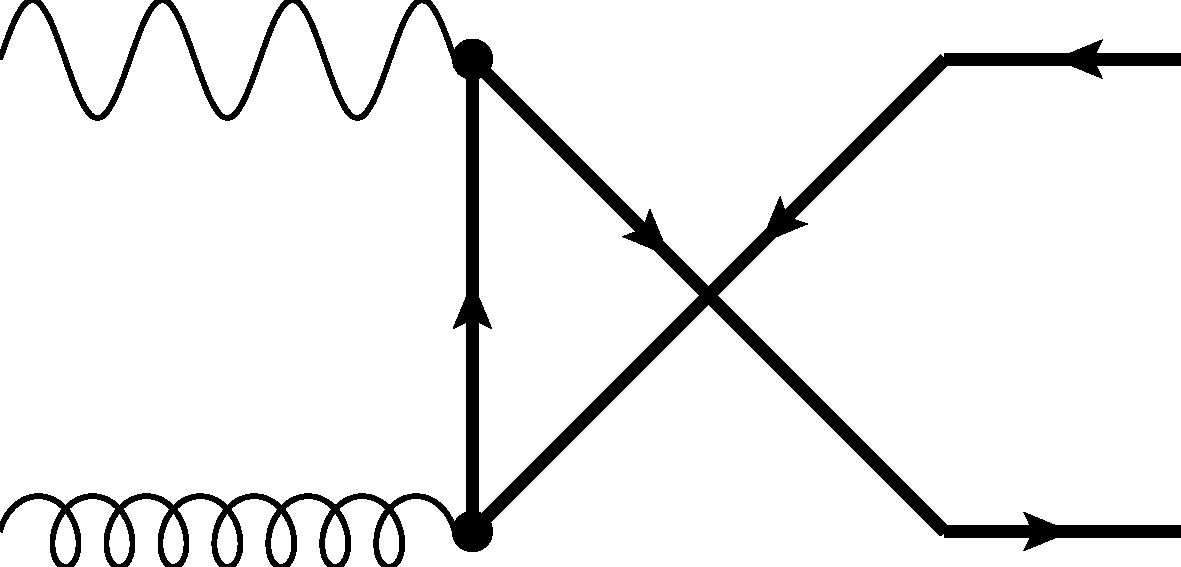
\includegraphics[width=\textwidth]{pyfeyn/lo-2}
	\caption{$i\varepsilon^{\mu}_{\Pgg}(q)\varepsilon^{\nu}_{\Pg}(k_1)\Md^{(0),2}_{\mu\nu}$}
\end{subfigure}
\caption{leading order Feynman diagrams}\label{fig:FeynLO}\fxerror{shift to appendix?}
\end{figure}

The result can then be written as
\begin{equation}
\hat {\mathcal P}_{k}^{\Pgg,\mu\mu'}\hat {\mathcal P}_{k}^{\Pg,\nu\nu'}\sum_{j,j'=1}^2\Md^{(0),j}_{\mu\nu}\left(\Md^{(0),j'}_{\mu'\nu'}\right)^* = 8g^2\mu_D^{-\epsilon}e^2e_H^2 N_C C_F B_{k,QED}
\end{equation}
where $g$ and $e$ are the strong and electromagnetic coupling constants respectively, $\mu_D$ is an arbitray mass parameter introduced to keep the couplings dimensionless and $e_H$ is the magnitude of the heavy quark in units of $e$. Further $N_C$ corresponds to the gauge group $SU(N_C)$ and the color factor $C_F=(N_C^2-1)/(2N_C)$ refers to the second Casimir constant of the fundamental representation for the quarks. We then find:
\begin{align}
B_{G,QED} &= \frac{t_1}{u_1} + \frac{u_1}{t_1} + \frac{4m^2s'}{t_1u_1}\left(1-\frac{m^2s'}{t_1u_1}\right)
+\frac{2s'q^2}{t_1u_1} +\frac{2q^4}{t_1u_1} + \frac{2m^2q^2}{t_1u_1}\left(2-\frac{{s'}^2}{t_1u_1}\right)\nonumber\\
 &\hspace{20pt}+\epsilon\left\{ -1 + \frac{{s'}^2}{t_1u_1} + \frac{s'q^2}{t_1u_1} -
\frac{q^4}{t_1u_1} - \frac{m^2q^2{s'}^2}{t_1^2u_1^2} \right\} + \epsilon^2\frac{{s'}^2}{4t_1u_1}\\
B_{L,QED} &= -\frac{4q^2}{s'}\left(\frac s {s'} - \frac{m^2s'}{t_1u_1}\right)\\
B_{P,QED} &= \frac 1 2\left(\frac{t_1}{u_1}+\frac{u_1}{t_1}\right)\left(\frac{2m^2 s'}{t_1u_1}-1 - \frac{2q^2}{s'}\right)\\
B_{k,QED} &= B^{(0)}_{k,QED} + \epsilon B^{(1)}_{k,QED} + \epsilon^2 B^{(2)}_{k,QED}
\end{align}

By using eq. (\ref{eq:PartonicStructureTensor0}) we can derive the $n$-dimensional $2\rightarrow 2$ phase space
\begin{equation}
dPS_2 = \!\int\!\!\frac{d^{n}p_1}{(2\pi)^{n-1}}\frac{d^{n}p_2}{(2\pi)^{n-1}}\Theta(p_{1,0})\delta(p_1^2-m^2)\Theta(p_{2,0})\delta(p_2^2-m^2)(2\pi)^n\delta^{(n)}(k_1+q-p_1-p_2)
\end{equation}
that can be solved by using the center-of-mass system (CMS) of the incoming particles\cite{Bojak:2000eu}
\begin{align}
q &= \left(\frac {s+q^2}{2\sqrt s},0,0,-\frac{s-q^2}{2\sqrt s},\hat 0\right) &
k_1 &= \frac {s-q^2}{2\sqrt s}\left(1,0,0,1,\hat 0\right)
\end{align}
such that $q+k_1=(\sqrt s,\vec 0)$ and $k_1^2 = 0$. For the outgoing particles it follows
\begin{align}
p_1 &= \frac{\sqrt s} 2 \left(1,0,\beta\sin\theta,\beta\cos\theta,\hat 0\right)&
p_2 &= \frac{\sqrt s} 2 \left(1,0,-\beta\sin\theta,-\beta\cos\theta,\hat 0\right)
\end{align}
such that $p_1+p_2 = (\sqrt s,\vec 0)$ and $p_1^2 = p_2^2=m^2$. Finally we have to use the $n$-sphere
\begin{equation}
d^nx = \frac{2\pi^{n/2}}{\Gamma(n/2)}x^{n-1} dx= \frac{\pi^{n/2}}{\Gamma(n/2)}(x^2)^{(n-2)/2} dx^2
\end{equation}
and arrive at the well known result\cite{Laenen1993162}
\begin{align}
dPS_2 &= \frac {\delta(s'+t_1+u_1)} {2s'\Gamma((n-2)/2)(4\pi)^{(n-2)/2}}\left(\frac{(t_1u_1'-s'm^2)s' - q^2t_1^2}{s'^2}\right)^{(n-4)/2}\,dt_1du_1\\
 &= \delta(s'+t_1+u_1) h_2(n)\,dt_1 du_1\\
h_2(4+\epsilon) &= \frac {2\pi S_\epsilon} {s'\Gamma(1+\epsilon/2)}\left(\frac{(t_1u_1'-s'm^2)s' - q^2t_1^2}{s'^2}\right)^{\epsilon/2}
\end{align}
with $S_\epsilon = (4\pi)^{(-2-\epsilon/2)}$.

The final double differential LO partonic cross section can then be written as
\begin{align}
{s'}^2\frac{d^2\sigma_{k,\Pg}^{(0)}(s',t_1,u_1,q^2)}{dt_1du_1} &= 2^6\alpha\alpha_s e_H^2 K_{\Pg\Pgg}N_CC_F E_k(\epsilon) b_k(\epsilon)\delta(s'+t_1+u_1) \frac{\pi^3S_\epsilon}{\Gamma(1+\epsilon/2)}  \nonumber\\
 &\hspace{20pt} \left(\frac{(t_1u_1'-s'm^2)s' - q^2t_1^2}{m^2{s'}^2}\right)^{\epsilon/2}\left(\frac{\mu_D^2}{m^2}\right)^{-\epsilon/2} B_{k,QED}
\end{align}
where we used $e^2=4\pi\alpha$ and $g^2=4\pi\alpha_s$. The color average is given by $K_{\Pg\Pgg} = 1/(N_C^2-1)$.

From the results above we can easily obtain the \textit{total} LO partonic cross sections
\begin{align}
\sigma_G^{(0)}(s,q^2,m^2) &=-4\pi\alpha\alpha_s e_H^2 K_{\Pg\Pgg}N_CC_F\frac 1 {{s'}^3}\left((s^2+q^4+4m^2 s)\beta + (s^2+q^4-4m^2(2m^2-s'))\ln(\chi)\right)\\
\sigma_L^{(0)}(s,q^2,m^2) &=16\pi\alpha\alpha_s e_H^2 K_{\Pg\Pgg}N_CC_F\left(\frac{-q^2s}{{s'}^3}\right)\left(\beta + \frac{2m^2}{s}\ln(\chi)\right)\\
\sigma_P^{(0)}(s,q^2,m^2) &=4\pi\alpha\alpha_s e_H^2 K_{\Pg\Pgg}N_CC_F\frac 1 {{s'}^2}\left((3s+q^2)\beta + (s+q^2)\ln(\chi)\right)
\end{align}
from which we also find
\begin{align}
\lim_{s\rightarrow 4m^2} \sigma_T^{(0)}(s',q^2) &= 4\pi\alpha\alpha_s e_H^2 K_{\Pg\Pgg}N_CC_F\frac{\beta}{4m^2-q^2} + O(\beta^3) = \lim_{s\rightarrow 4m^2} \sigma_P^{(0)}(s',q^2)\\
\lim_{s\rightarrow 4m^2} \sigma_L^{(0)}(s',q^2) &= -\frac{128}{3}\pi\alpha\alpha_s e_H^2 K_{\Pg\Pgg}N_CC_F\frac{m^2q^2\beta^3}{(4m^2-q^2)^3} + O(\beta^5)
\end{align}
(Note the missing factor of 2 in \cite[eq. (5.9)]{Laenen1993162}.)
\fxerror{shift to partonic?}
